\chapter{SMEE Performance}
\label{chp:performance}

This chapter will summarize the performance of SMEE as a parameter estimation tool. A sample of results from SMEE's code review will be presented, an example case study will be performed, and future detector configurations will be simulated in order to gauge how SMEE's performance will improve over the coming decades.

\section{SMEE Code Review}

SMEE is currently under review in order to be added to LIGO's official run plan for GW signals from CCSNe. Different aspects of SMEE's algorithm have been tested and some of those results will be presented in this section.

As discussed in section~\ref{sec:PCA}, performing PCA on spectrograms means chopping up the columns of a spectrogram, combining those columns into one long vector, running the PCA algorithm on said vector, and then reassembling everything back into a spectrogram for later use. The first simple test was to examine the effects of reordering the columns before PCA. In short, this had no effect on the PCs produced. As long as the PC vector was chopped up and reassembled in a consistent fashion (so that the final spectrogram was in the proper order), there was no discernible impact on the PCs. The original PCs and the reordered PCs also produced identical Bayes factors for identical injections.

\begin{figure*}[t!]
\centering
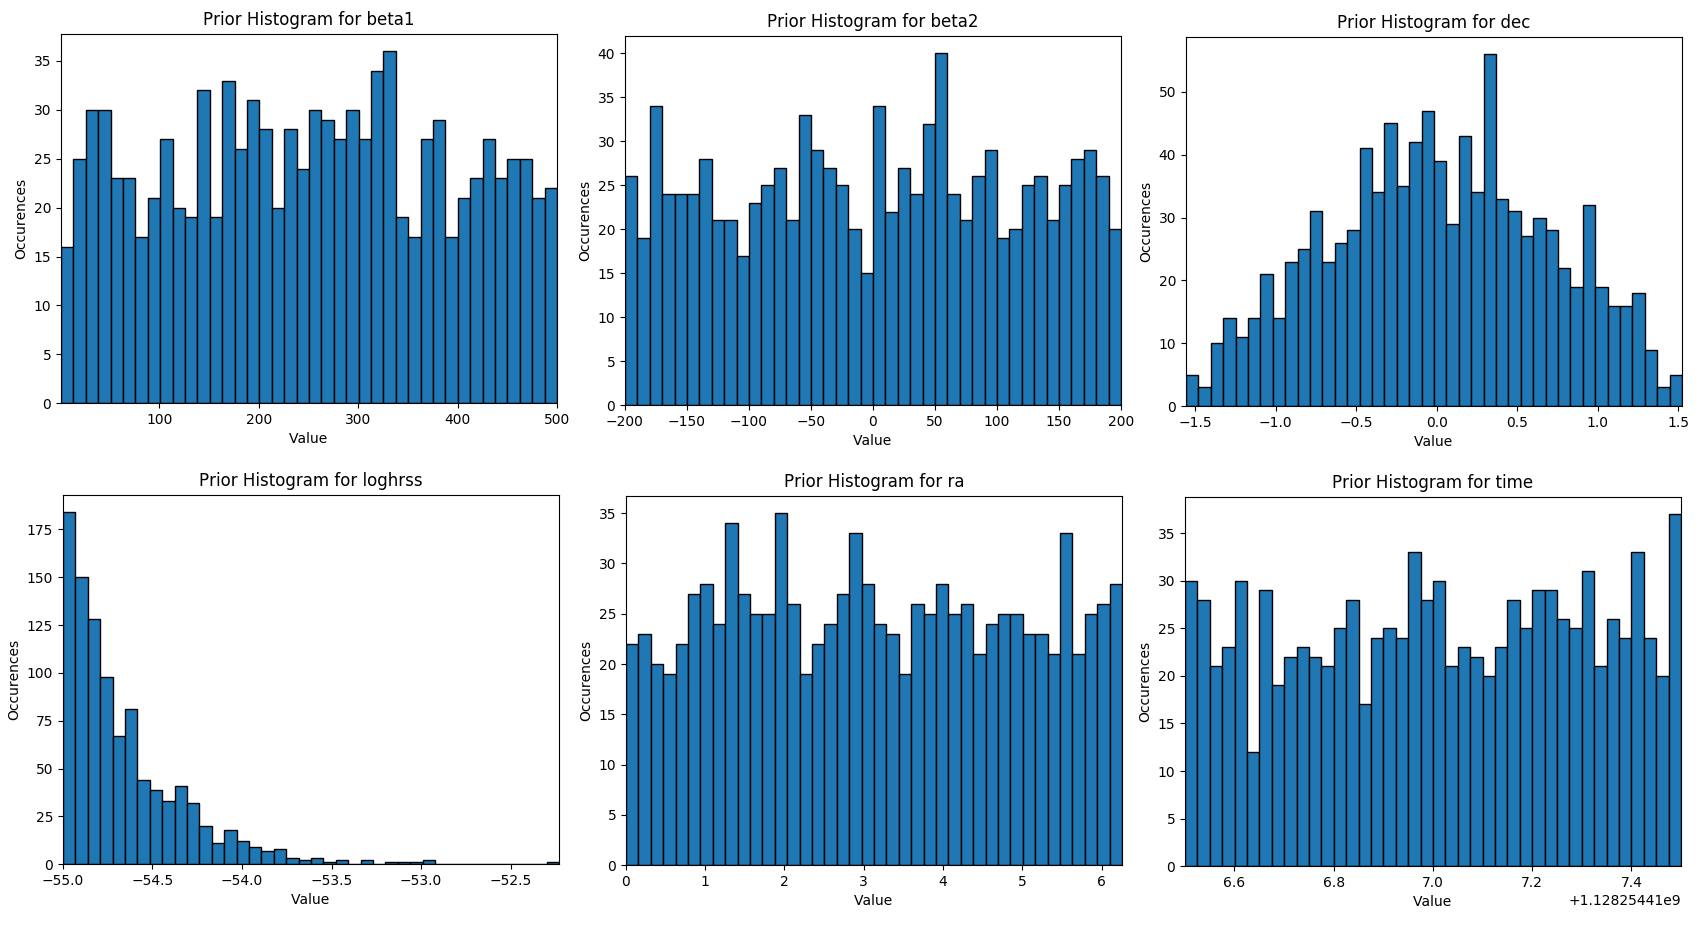
\includegraphics[width=\textwidth]{figures/priors.png}
\caption{Six prior distributions within SMEE. The prior for declination is uniform in cosine, the prior for $\log h_{rss}$ is uniform in volume, and the remaining priors are flat.}
\label{fig:priors}
\end{figure*}

The prior distributions within SMEE were also tested and can be seen in Figure~\ref{fig:priors}. Most of SMEE's parameters have a flat, uniform prior distribution. SMEE's priors are discussed in section~\ref{sec:priors}. The priors behaved as expected when tested.

The performance of SMEE when running on noise (no CCSN signal) is extremely important. CCSN searches are typically triggered by electromagnetic and neutrino observations. A window of data is then selected to represent the possible arrival time of a GW. This window is searched for excess power events that are coherent between detectors. It is important that SMEE does not see CCSN signals in the data when they are not genuinely present. To test this, SMEE was ran 1000 times on randomly chosen segments of O1 data. This was performed with the neutrino and magnetorotational PCs. All of these trials produced negative $\log B_{S,N}$ values, indicating that no signals were detected. These results are shown in Figure~\ref{fig:noise_runs}.

\begin{figure*}[t!]
\centering
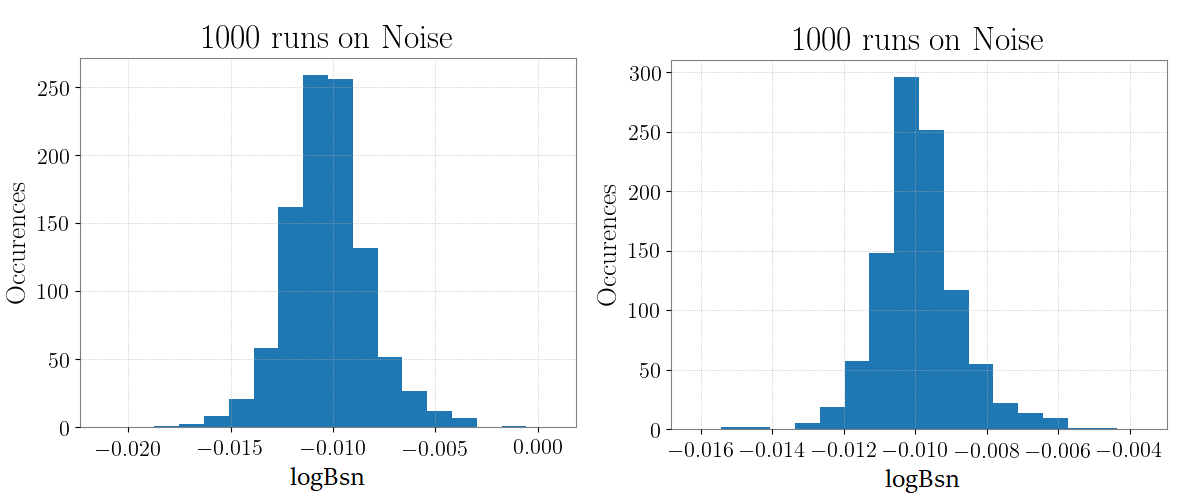
\includegraphics[width=\textwidth]{figures/noise_runs.png}
\caption{Left: Noise performance with Neutrino model PCs. Right: Magnetorotational PCs. All tests were performed on O1 data with no injections.}
\label{fig:noise_runs}
\end{figure*}

\section{Reconstructions}

This section contains example SMEE reconstructions with different sets of PCs. All injections were performed from 3\,-\,5\,kpc with a known sky position into a simulated future detector configuration with two A+ detectors, one Advanced Virgo detector, and one Kagra detector. For the mechanism classification reconstructions, all injections were non-catalog waveforms. This was not the case for waveform feature classification due to a limited number of waveforms.

\begin{figure*}[p]
    \centering
    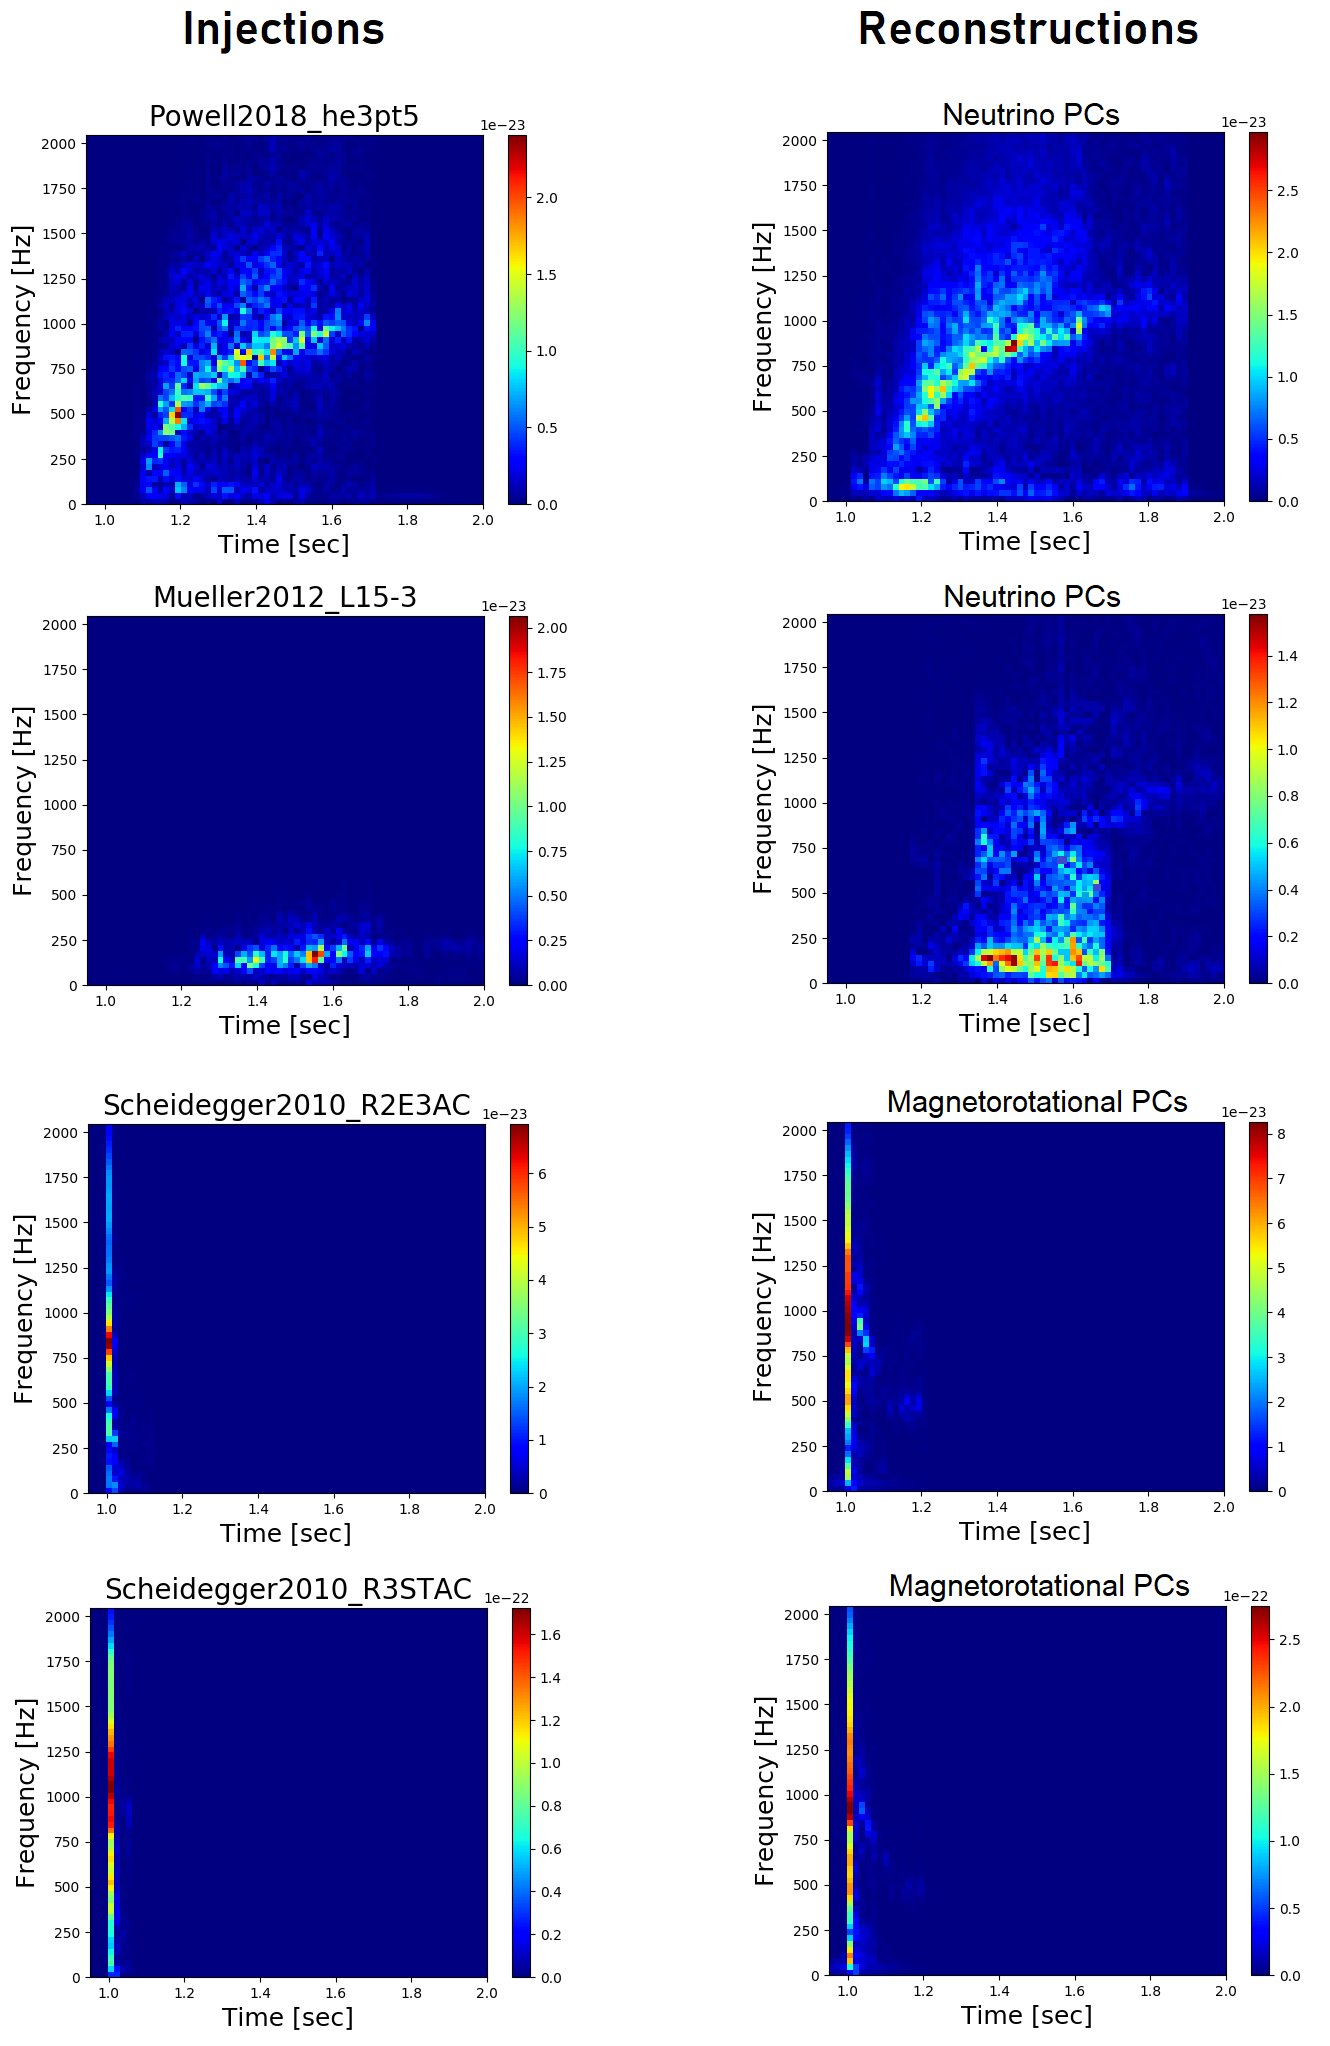
\includegraphics[height=8.3in]{figures/mechanism_reconstructions.png}
    \caption{Example reconstructions for mechanism classification PCs.}
    \label{fig:mechanism_reconstructions}
\end{figure*}

\begin{figure*}[p]
    \centering
    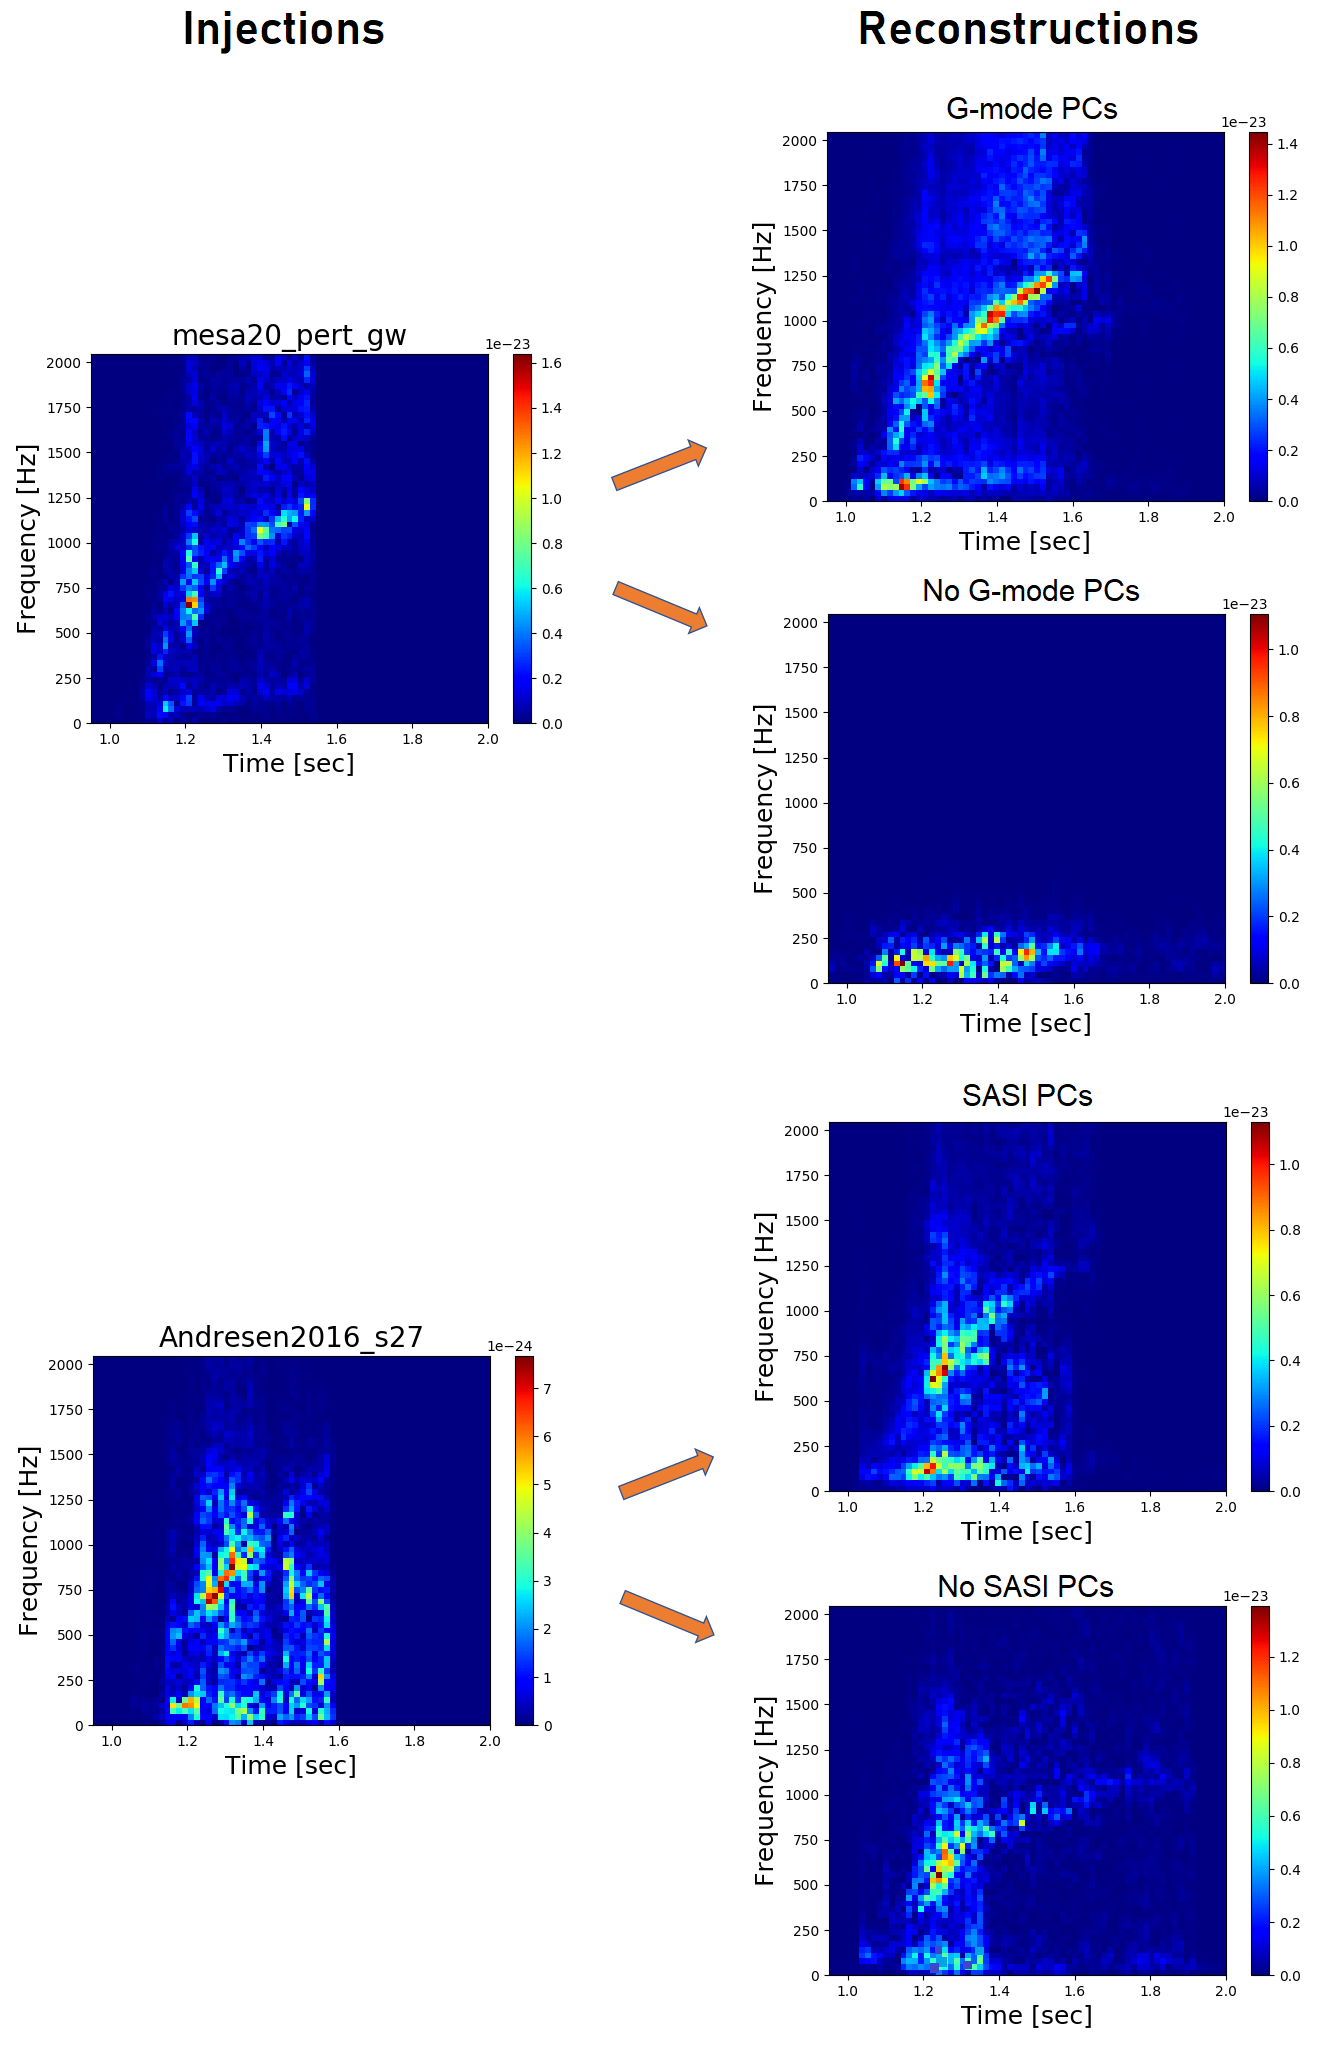
\includegraphics[height=8.3in]{figures/feature_reconstructions.png}
    \caption{Example reconstructions for waveform feature classification PCs.}
    \label{fig:feature_reconstructions}
\end{figure*}

Reconstructions with mechanism classification PCs are shown in Figure~\ref{fig:mechanism_reconstructions}. Reconstructions with waveform feature PCs are shown in Figure~\ref{fig:feature_reconstructions}. For the mechanism classification PCs, only reconstructions with the ``correct" PCs, the PCs that match the injection type, are displayed. All injections reached the Bayes factor threshold for confident classification.

\section{Example Case Study}

\begin{figure*}[b!]
\centering
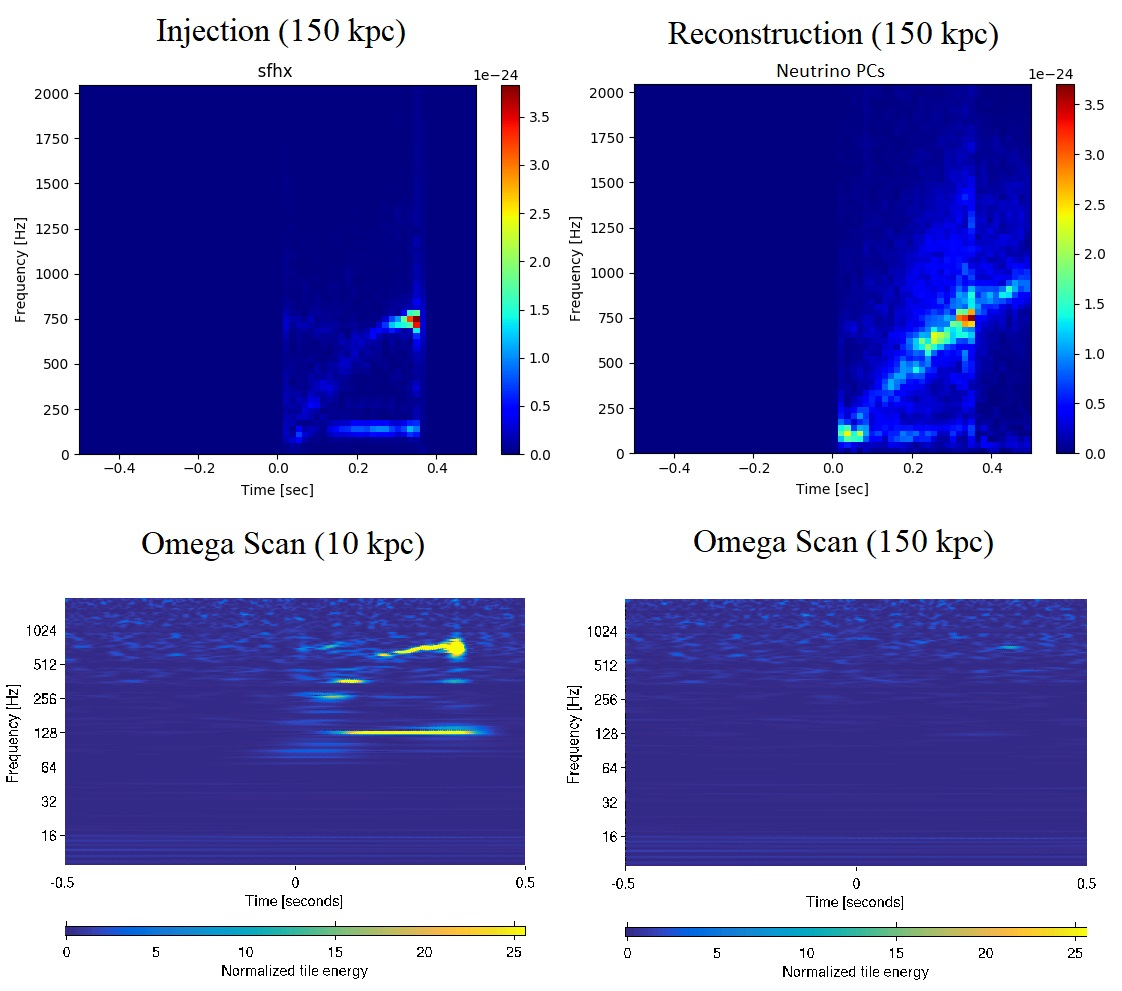
\includegraphics[width=15cm]{figures/Reconstruction_Plot_8.jpg}
\caption{Top row shows injected waveform and waveform reconstruction produced with the neutrino model PCs at 150\,kpc in three ET and two Voyager detectors. Bottom row shows Omega Scan spectrograms of the data from the detector in the configuration with the highest SNR. Bottom left plot shows the signal is clearly visible by eye for a 10\,kpc injection (SNR = 120), while the bottom right plot shows almost nothing visible at 150\,kpc (SNR = 8). This waveform was confidently classified at 150\,kpc as corresponding to the neutrino model with g-mode and SASI emission, even though at that distance those features are clearly not visible by eye in the noisy Omega scan.}
\label{fig:recon}
\end{figure*}

This section will summarize an example case study in which model sfhx was injected into a simulated configuration with three ET detectors and two Voyager detectors. The signal was injected at a distance of 150\,kpc using an arbitrary sky position. The resulting network SNR was 11.4\,. The injected waveform, an example reconstruction, and example Omega Scans of one detector's data are shown in Figure~\ref{fig:recon}. Omega scans are commonly used spectrograms to view detector data within the LIGO collaboration~\cite{chatterji2004multiresolution}. All three classification statements were performed on the signal. With the neutrino model PCs, the result was $\log B_{S,N} = 55.5\,$. With the magnetorotational PCs the result was $\log B_{S,N} = 1.5\,$. This gives a final mechanism classification result of $\log B_{neu,mag} = 54\,$. This result is well above the confidence threshold and tells us that our signal matches the neutrino model much more strongly than the magnetorotational. Because it appears to be a slowly rotating neutrino model waveform, the two waveform feature classification statements can be performed.

For g-mode and SASI classification, the g-mode PCs gave a result of $\log B_{S,N} = 62.7\,$, while the no g-mode PCs gave $\log B_{S,N} = 1.3\,$. Subtracting the two gives the final g-mode result of $\log B_{gmode,\,no\,gmode} = 61.4\,$. This is also well above the confidence threshold and tells us strongly that high frequency g-modes were present in the signal. The SASI PCs gave a result of $\log B_{S,N} = 97.7\,$ while the no SASI PCs gave $\log B_{S,N} = 61.8\,$. This gives the final result for SASI classification, $\log B_{SASI,\,no\,SASI} = 35.9\,$. This is also above the confidence threshold and tells us that low frequency SASI signals were present in the data. For this simulated CCSN signal, all three classification statements were made with a high confidence level even though the network SNR of the signal is relatively low and the signal features are clearly not visible in the noisy spectrogram shown in Figure~\ref{fig:recon}. % When the same model is injected with an SNR of 23, at half that distance considered in this example, almost the entire waveform is still not visible in an Omega Scan of the detector data.

\section{Minimum SNR}

\begin{figure*}[b!]
\centering
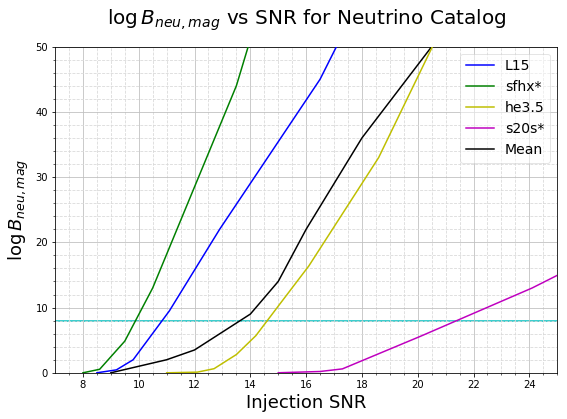
\includegraphics[width=2.75in]{figures/SNR_neu.png}
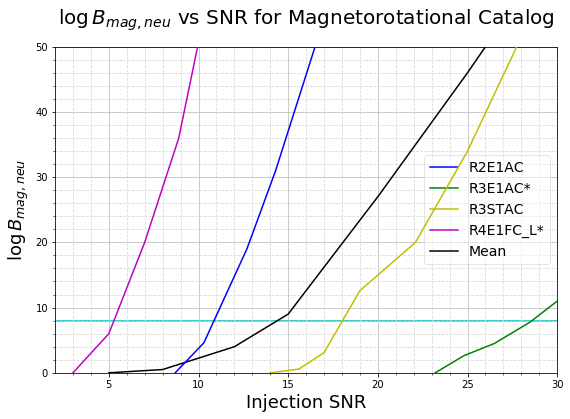
\includegraphics[width=2.75in]{figures/SNR_sch.png}
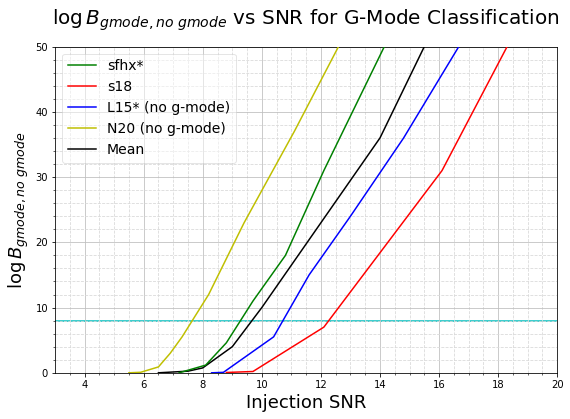
\includegraphics[width=2.75in]{figures/SNR_gmode.png}
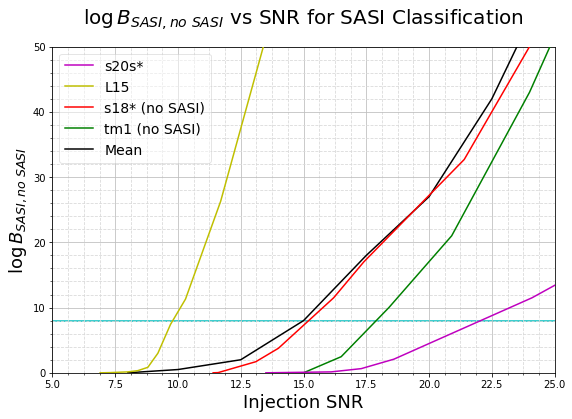
\includegraphics[width=2.75in]{figures/SNR_sasi.png}
\caption{Minimum detectable SNR for each classification statement. All injections performed in a simulated A+ configuration that included Advanced Virgo and Kagra. The top two plots both pertain to mechanism classification, and the bottom two are for g-modes and SASI. Models with an asterisk (*) were not included in the PCA. All results are organized such that positive Bayes values correspond to correct classifications regardless of whether the feature is present or not.}
\label{fig:min_snr}
\end{figure*}

The top two panels in Figure~\ref{fig:min_snr} show the mechanism classification performance for neutrino and magnetorotational waveforms as a function of injected network SNR. All SNR plots were created while running SMEE on a simulated A+ configuration that will be described in Section~\ref{subsec:eras}. On average, neutrino model waveforms needed an SNR of about 14 or greater to be confidently classified. Some waveforms, such as s20s, required an SNR in the low twenties. This is likely due to the fact that this waveform's peak frequency of emission is around 100\,Hz and the short PSDs in SMEE's spectrograms are hindered by the 60\,Hz mains power peak present in Advanced LIGO's data. This can lower our sensitivity to signal energy in the vicinity of 60\,Hz. Magnetorotational waveforms performed similarly and also had an average minimum SNR of about 14, with one plotted waveform requiring an SNR above 28. Despite the similar minimum SNRs, magnetorotational waveforms are generally easier to resolve at a given distance due to their larger signal energies. 

The bottom two panels in Figure~\ref{fig:min_snr} show SMEE's performance as a function of SNR for SASI and g-mode classification. The average minimum SNR required to make statements about the presence of g-modes was just below 9, while the average minimum for SASI statements was 15. Similarly to mechanism classification, s20s required the largest SNR of about 22 in order to confidently say that SASI was present. This is, again, likely due to SMEE's hindered sensitivity around 60\,Hz. It was generally similarly difficult for SMEE to determine that a feature was present than to rule it out, with both cases sometimes performing better.

\section{Methodology for Testing Future Detectors}

The analysis presented in this section was designed to test SMEE's effectiveness in future detector arrangements. Specifically, the ability to distinguish between explosion mechanisms (neutrino vs magnetorotational) along with the ability to make statements about the presence of predicted waveform features (SASI and g-modes) in an observed signal. Future detector data is simulated as realistically as possible by adjusting segments of Advanced LIGO's O1 data to match the estimated sensitivity curves of future detectors in a process called ``recoloring". We can then ``inject" a waveform by inserting its time series into the detector data. We inject CCSN waveforms over the entire sky at different GPS-times and with different orientations in order to test SMEE's performance on emissions from an unknown, possibly extra-galactic source. The results of these tests will be presented in section~\ref{sec:performance}.

\subsection{Recoloring}

\begin{figure}[b!]
\centering
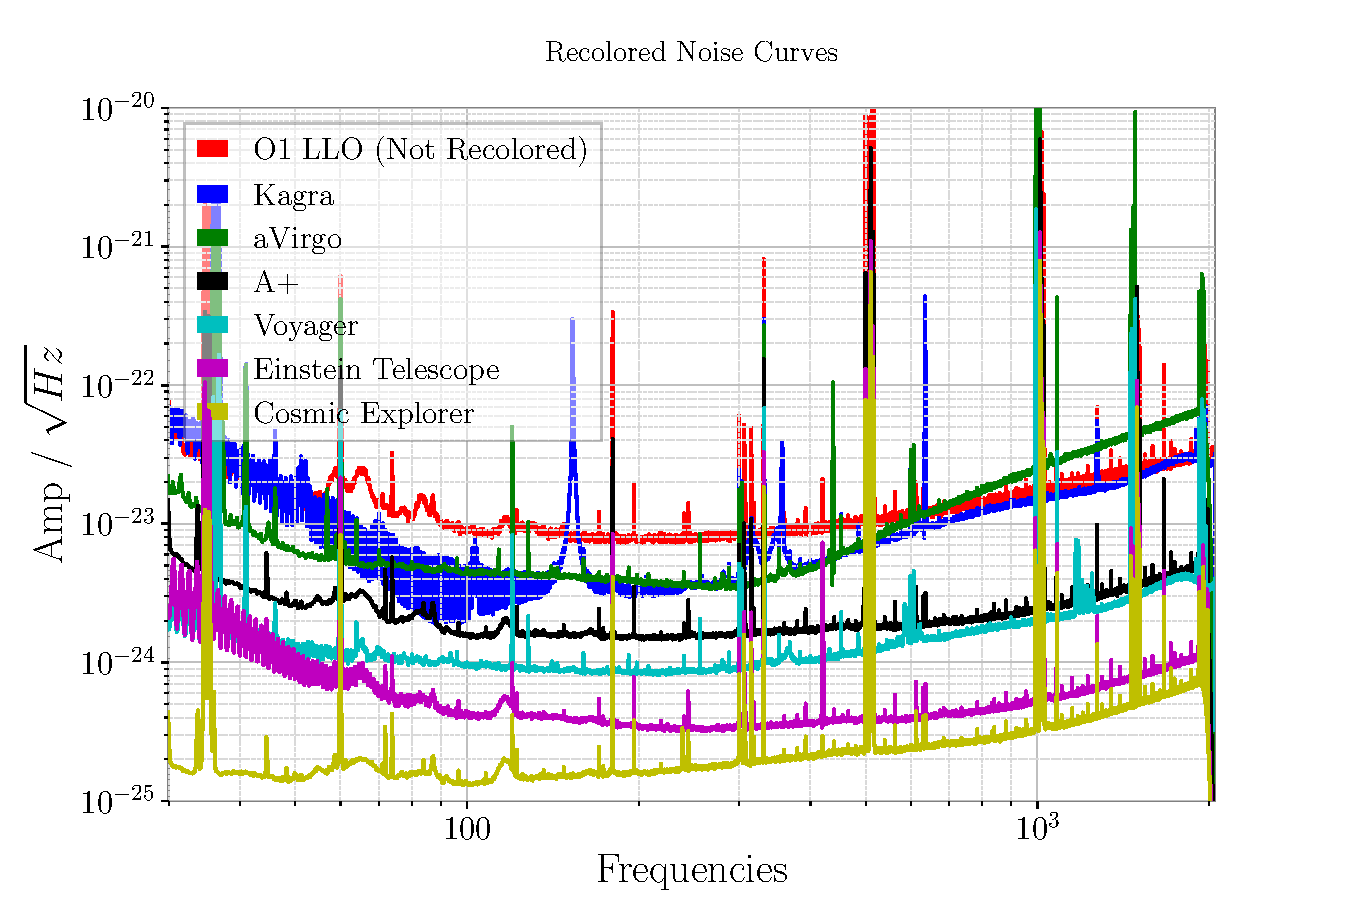
\includegraphics[width=\textwidth]{figures/recolored_noise_curves.pdf}
\caption{Spectra for LIGO O1 data recolored to future detector sensitivities. Data is shown from 30 - 2048 Hz, the frequency band used in SMEE's analysis.}
\label{fig:recolored_curves}
\end{figure}

Six different 24 hour segments of data from Advanced LIGO's first observing run (O1) were chosen to be recolored. Recolored data possesses the calibration lines and transient noise glitches not found in simulated Gaussian data. The recoloring was performed with the GSTLAL software package~\cite{messick2017analysis}. GSTLAL contains software for data manipulation and the generation of simulated data. In this case, each segment of data was whitened with a reference PSD and then recolored with a filter to the noise curves of future detectors. The noise curves for the recolored data are shown in Figure~\ref{fig:recolored_curves}. Cosmic Explorer is the most sensitive detector considered in this study. After recoloring, each segment of data was reassigned to start at GPS time 1128211934. One segment of data, starting at 1132759948, contained O1 data from Livingston, while the other five (epochs: 1128211934, 1135238505, 1128618400, 1129037417, 1130767217) contained data from Hanford. All of the O1 data used is available from the Gravitational Wave Open Science Center (GWOSC)~\cite{2015JPhCS.610a2021V}.

\subsection{Detector Eras}
\label{subsec:eras}

Future detector configurations have been simulated over the next few decades. All predicted dates of operation are rough estimates that may change significantly. The first configuration consists of LIGO A+ (2), Advanced Virgo, and Kagra. Advanced Virgo is already operational and will join the two Advanced LIGO detectors for the next Observing Run in 2019~\cite{AdVirgo}. Kagra is also expected to come online in the near future and may participate in O3~\cite{2013PhRvD..88d3007A, Somiya2012detector, aso2013interferometer}. The funding for LIGO A+ has been approved and this three detector configuration should be operational by approximately 2022. The second configuration is similar but upgrades each LIGO detector. It has LIGO Voyager (2), Advanced Virgo, and Kagra. These detectors are expected to be operational between the period of 2024\,-\,2028. The third configuration is identical but adds a third Voyager detector located in India. An interferometer is planned for India~\cite{unnikrishnan2013indigo} but it is unknown precisely what technology will be included or what sensitivity it will have upon arrival.

The fourth configuration consists of the triangular Einstein Telescope (3) in Europe and two Voyager detectors at the current LIGO sites. The Einstein Telescope represents the first truly 3rd Generation detector~\cite{0264-9381-27-19-194002, ET:design}. Because it is a triangular detector, the single site will operate three interferometers. The Einstein Telescope may be operational by 2027. The fifth and final configuration consists of Cosmic Explorer and the Einstein Telescope (3). This configuration contains only 3rd Generation detectors and will require LIGO to obtain a new construction site as neither current location is large enough for the 40\,km arms~\cite{2017CQGra..34d4001A, whitepaper2018}. This configuration may be operational by $\sim2037$ but will depend on many factors.

\subsection{Injection and Sky Patterns}

Previous SMEE papers have examined performance from galactic sources, usually injecting signals from the galactic center's sky position~\cite{powell:16b, 2017PhRvD..96l3013P}, but future detectors will likely be sensitive to CCSN sources well outside of our own Galaxy~\cite{0264-9381-27-19-194002, 2017CQGra..34d4001A}. Because of this, waveforms are injected from six positions evenly distributed over the entire sky to test performance from an arbitrary source. At each sky location, injections are performed with three different polarization angles (0,\,$\pi/3$,\,$2\pi/3$) evenly distributed throughout the possible parameter space. This is done at five different GPS times evenly distributed throughout a 24 hour period to account for Earth's rotation and the detectors' changing antenna patterns. Injections are performed at 5 GPS times, with 6 different sky locations, and with 3 different polarization angles. That means that for each signal model, each waveform is injected 90 times at each distance. This gives a reasonable sample of results to gauge performance from an unknown source. The injections are performed for each detector era and configuration described in the previous section.

\subsection{Mechanism Classification}

Two waveforms were omitted from the neutrino catalog and the magnetorotational catalog during the creation of the signal models. Any real life CCSN signal we observe will, of course, not identically resemble any simulated waveform in the catalog, therefore these omitted non-catalog waveforms serve as a more realistic test of a genuine signal. For the catalog waveforms (waveforms included in the PCA), four were selected from each catalog and injected as described in the previous paragraphs. For the neutrino catalog, s20s, tm1, C15, and s18 were selected from different simulation groups. All of the magnetorotational waveforms came from the Scheidegger group, so the four chosen, R2E1AC, R3E1DB, R3STAC, and R4STAC, were evenly distributed between the minimum and maximum signal energies of the catalog. We define efficiency at a given distance as the fraction of injected waveforms that could be correctly identified with a log Bayes factor above our confidence threshold. The remaing injections could not be confidently classified. For this analysis, our confidence threshold was $\log B_{i,j} \geq 8$~\cite{powell:16b, 2017PhRvD..96l3013P}.

\subsection{Presence of SASI/G-modes}

Two non-catalog waveforms were injected for each waveform feature. One waveform has the feature and the other does not. The waveforms were injected in the manner described above and the same confidence threshold was used ($\log B_{i,j}~\geq~8$). Regardless of whether the feature was present or not, the Bayes factors will be oriented such that positive answers are the correct answers. As an example, for an injection containing a g-mode signal, $\log B_{gmode,\,no\,gmode}\,$ would be calculated, whereas for an injection containing no g-mode signal, $\log B_{no\,gmode,\,gmode}$ would be calculated. This allows related results to be presented in one simple figure.

\section{Future Detector Performance}
\label{sec:performance}

\subsection{Mechanism Classification}
\label{subsec:mechanism_range}

\begin{figure*}[b!]
\centering
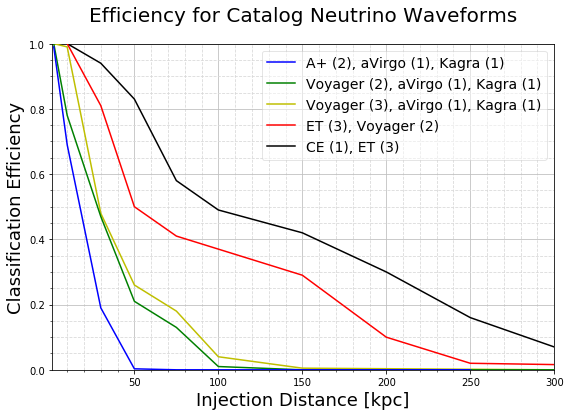
\includegraphics[width=2.75in]{figures/neu_eff_cat.png}
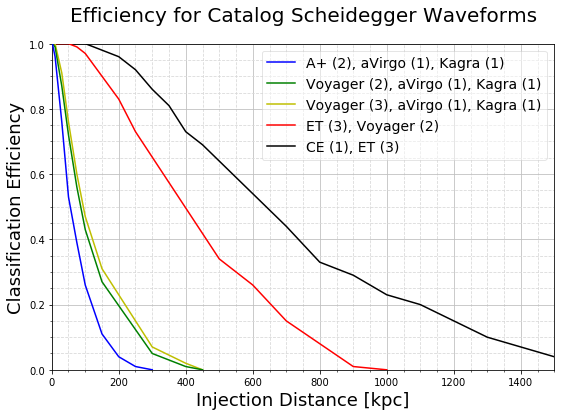
\includegraphics[width=2.75in]{figures/sch_eff_cat.png}
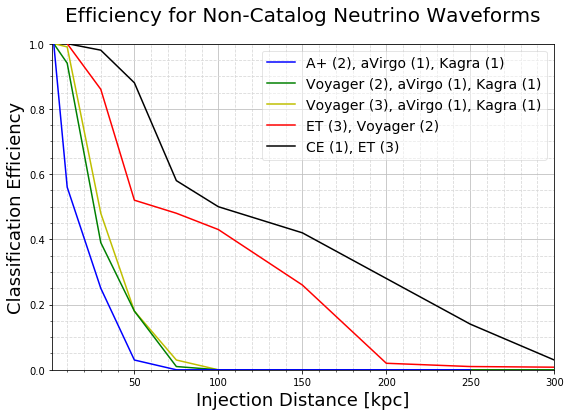
\includegraphics[width=2.75in]{figures/neu_eff_nonc.png}
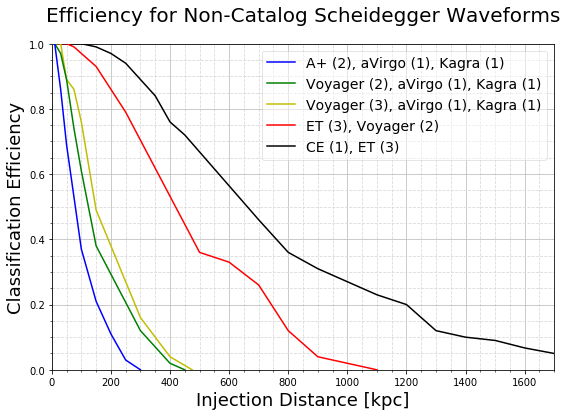
\includegraphics[width=2.75in]{figures/sch_eff_nonc.png}
\caption{Mechanism classification efficiency. Top plots show results for catalog waveform injections, bottom plots show results for non-catalog injections. Non-catalog injections are considered to be the most realistic test case for a genuine gravitional wave signal from an arbitrary source.}
\label{fig:eff_mech}
\end{figure*}

SMEE's ability to determine a source's explosion mechanism is shown in Figure~\ref{fig:eff_mech} for both catalog waveform injections and non-catalog injections. The performance differs greatly when injecting magnetorotational model waveforms vs injecting neutrino model waveforms due to the former having greater energy levels. For both explosion mechanism models, the non-catalog performance is very similar to that of catalog waveforms. The fact that non-catalog performance is on par with catalog performance is a testament to the robustness of SMEE's spectrogram format. 

All future detector arrangements were able to confidently classify magnetorotational injections well beyond the limits of the Milky Way, with the third generation detectors confidently classifying about 50\% of injections at a distance of 400\,-\,700\,kpc and 10\% of injections at a distance of 1.5\,Mpc. For neutrino model waveforms, all future detector arrangements performed with greater than 56\% efficiency at 10\,kpc, suggesting that the explosion mechanism of a galactic CCSN would likely be confidently classified. Low energy explosions, and explosions originating from unfortunate sky positions, could still fail to be classified from within our galaxy in LIGO's A+ configuration. Only 2\,-\,5\% of galactic injections failed to be confidently classified in Voyager configurations. Adding a third Voyager detector improves coverage and efficiencies at close distances, but does little to increase SMEE's range. All galactic injections were confidently classified in the ET and Cosmic Explorer arrangements. Third generation detectors had a 50\% efficiency for neutrino model waveforms at a distance of 100\,-\,150\,kpc. There are 28 known galaxies within a range of 150\,kpc and 55 within a range of 790\,kpc~\cite{karachentsev2004catalog, belokurov2007cats}, suggesting that a CCSN detection and classification is very plausible over the next few decades.

\subsection{Waveform Features}
\label{subsec:features_future}

SMEE's ability to detect g-modes and SASI is shown in Figure~\ref{fig:eff_features}. The figure shows the efficiencies for all injections, half of which contained the waveform feature and half of which did not. In general the performance is similar to that of neutrino model waveforms for mechanism classification. At 10\,kpc in our simulated A+ arrangement, the SASI and g-mode classification efficiencies were 63\% and 56\% respectively, suggesting that these statements would likely reach the confidence threshold for a galactic CCSN. These results suggest that when the ET or Cosmic Explorer detectors are operational, it should be possible to determine if g-modes or SASI are present in galactic CCSN signals even if they occur in a part of the sky with poor detector sensitivity. Waveform feature performance in third generation detectors is similar to that of neutrino mechanism classification, with a 50\% efficiency in the range of 100\,-\,150\,kpc. 

\begin{figure*}[t!]
\centering
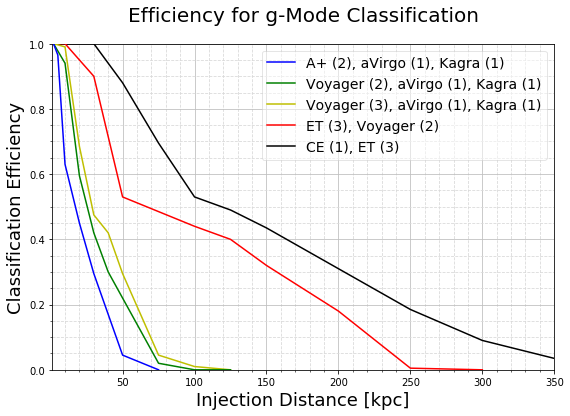
\includegraphics[width=2.75in]{figures/eff_gmode.png}
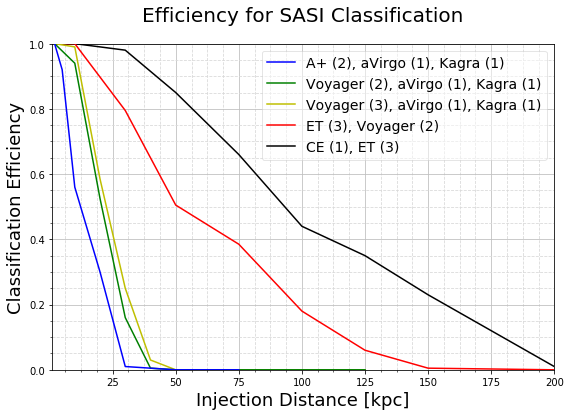
\includegraphics[width=2.75in]{figures/eff_sasi.png}
\caption{Classification efficiency for g-mode (left) and SASI (right) waveform features. Performance was better for g-mode classification in our tests, but this is also heavily dependent on the energy of the specific waveform. Overall performance was similar to that of neutrino model mechanism classification.}
\label{fig:eff_features}
\end{figure*}